\documentclass[twoside]{article}
\usepackage{aistats2022}
% If your paper is accepted, change the options for the package
% aistats2022 as follows:
%\usepackage[accepted]{aistats2022}

% If you set papersize explicitly, activate the following three lines:
%\special{papersize = 8.5in, 11in}
%\setlength{\pdfpageheight}{11in}
%\setlength{\pdfpagewidth}{8.5in}

% If you use natbib package, activate the following three lines:
\usepackage[round]{natbib}
\renewcommand{\bibname}{References}
\renewcommand{\bibsection}{\subsubsection*{\bibname}}

\usepackage[utf8]{inputenc} % allow utf-8 input
\usepackage[T1]{fontenc}    % use 8-bit T1 fonts
\usepackage{hyperref}       % hyperlinks
\usepackage{url}            % simple URL typesetting
\usepackage{booktabs}       % professional-quality tables
\usepackage{microtype}      % microtypography
\usepackage{graphicx}
\graphicspath{{../figs/}}
%\usepackage{subfigure}
\usepackage{subcaption}
\usepackage{hyperref}       % hyperlinks
\usepackage[dvipsnames]{xcolor}

\hypersetup{ % SLJ: my standard paper setup...
	pdftitle={MAP convergence},
	pdfkeywords={},
	pdfborder=0 0 0,
	pdfpagemode=UseNone,
	colorlinks=true,
	linkcolor=blue, %mydarkblue,
	citecolor=blue, %mydarkblue,
	filecolor=blue, %mydarkblue,
	urlcolor=blue, %mydarkblue,
	pdfview=FitH,
	pdfauthor={Anonymous},
}


\newcommand{\RLP}[1]{\textcolor{red}{RLP:#1}}
\newcommand{\TODO}[1]{\textcolor{cyan}{TODO #1}}

% my packages
\usepackage{../math_commands}
% some custom math commands
\newtheorem{proposition}{Proposition}
\newcommand*{\expect}[2][]{\ensuremath{\mathbb{E}_{#1} \left[ #2 \right] }} % expectation operator
\newcommand{\logpart}{A}
\newcommand{\conj}{\logpart^*}
\newcommand{\bregman}{\cB_\logpart}
\newcommand{\bregmanconj}{\cB_{\logpart^*}}
\newcommand{\natp}{\theta}
\newcommand{\meanp}{\mu}
\newcommand{\decrement}{D}
\newcommand{\linear}{\ell} % linearization of a function
\newcommand{\lr}{\gamma} % learning rate, or step-size

\newcommand{\MAPm}{\hat \mu_n}
\newcommand{\MAPt}{\hat \natp_n}


\begin{document}

% If your paper is accepted and the title of your paper is very long,
% the style will print as headings an error message. Use the following
% command to supply a shorter title of your paper so that it can be
% used as headings.
%
%\runningtitle{I use this title instead because the last one was very long}

% If your paper is accepted and the number of authors is large, the
% style will print as headings an error message. Use the following
% command to supply a shorter version of the authors names so that
% they can be used as headings (for example, use only the surnames)
%
%\runningauthor{Surname 1, Surname 2, Surname 3, ...., Surname n}

\twocolumn[

\aistatstitle{Looking for Convergence Rates\\ for the MAP of the Exponential Family}


\aistatsauthor{R\'emi Le Priol \And Frederik Kunstner \And  Damien Scieur \And Simon Lacoste-Julien }

\aistatsaddress{ Mila \And  UBC \And SAIT SAIL \And Mila} 
]

\begin{abstract}
We raise the problem of upper bounding the expected sub-optimality of the maximum likelihood estimate, or a conjugate maximum a posteriori for the exponential family. 
Surprisingly, we found no solution to this problem in the literature -- we are not able to tell how many samples we need to fit a gaussian within a few bits of the true distribution.
After displaying some properties and special cases of this problem, 
we show it is a special case of several optimization algorithms, but it falls out of their scopes, thus highlighting range of progress in the analysis of these algorithms.
\end{abstract}

\section{Plan}

\begin{enumerate}
	\item intro to exponential family, and density estimation
	\item the thing we want to bound
	\item Examples : gaussian mean and gaussian variance (+other examples, just mentioned)
	\item Insight : Strongly convex case. (+ self-concordance that is not verified either)
	\item insight : bias-variance decomposition
	\item Optimization perspective : SBPP or SBG. But no analysis hold, revealing a flaw of all these techniques.
	\item Discussion : we believe finding a convergence rate would bring new tools useful to deal with common objects such as barrier losses.
\end{enumerate}

Open questions
\begin{itemize}
	\item does a base measure change anything ?
	\item is there multiple conjugate priors ?
	\item misspecified case. Do we have a   formula ?
	\item make sure the gaussian entropy is not SC.
\end{itemize}

\section{Introduction and Background}
\RLP{Goal = disseminate related work to make it look nice.}
Exponential Families are an elegant and lean way to model a wide variety of data : binary, categorical, natural numbers, positive float, long or short tailed... 
They are literally the linear model of probabilities.
The exponential family for data $X\in\cX$  with sufficient statistic $T$ and natural parameter $\natp$ is the model 
\begin{equation}
	 p(X|\natp) = \exp( \natp^\top T(X) - \logpart(\natp)) \; ,
\end{equation}
where $\logpart$ is the log-partition function -- i.e. the normalization factor
\begin{align}
    \logpart(\natp) = \log \int e^{\natp^\top T(x)} dx 
\end{align}
where the integral stands for a sum if $x$ has discrete support. \RLP{Use base measure instead.}
Note that an exponential family is entirely specified by its support set $\cX$ and its sufficient statistic $T$.
This simple model encompasses both categorical distributions $\cX = \{1, \dots, k\}$ with $T(X)$ being the one-hot encoding, and multivariate normal distributions $\cX=\real, T(X)=(X, X^2)$. 

\paragraph{Duality}
The logpartition function $\logpart$ verifies the two following identities
\begin{align}
    \nabla\logpart(\natp) &=  \expect[p(X|\natp)]{T(X)} =: \meanp \\
    \nabla^2 \logpart(\natp) &= \Cov_\natp[T(X)] > 0
\end{align}
where $\meanp$ is called the mean parameter.
If the sufficient statistic $T$ is minimal, then the log-partition function $\logpart$ is strictly convex and its gradient $\nabla \logpart$ is a bijection between natural parameters $\natp$ and mean parameters $\mu$.
The second identity entails that $\logpart$ is strictly-convex. 
At this point it is useful to introduce the \href{https://en.wikipedia.org/wiki/Convex_conjugate}{convex conjugate} (aka Fenchel-Legendre transform) of the logpartition function
\begin{align}
	\conj(\mu) = \langle \mu, \natp \rangle - \logpart(\natp) \; .
\end{align}
It turns out that $\conj$ matches the common notion of \textit{entropy} in information theory, so we will call it entropy.
If $\logpart$ is strictly convex, then its gradient is strictly monotone, so it is a bijection, and its inverse is the gradient of its dual $\nabla\conj \circ \nabla\logpart(\natp) = \natp$ (cf Fig.~\ref{fig:duality}).
For a full review of exponential families and their duality, see \citet[Chapter 3]{wainwright2008graphical}.
\begin{figure}[ht]
	\centering
	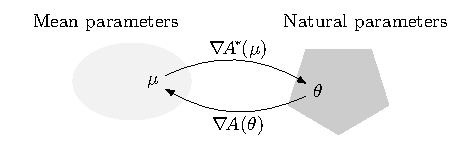
\includegraphics{duality}
	\caption{The gradient of the log-partition function and its dual, $(\nabla \logpart, \nabla \conj)$, form a bijection between the natural and mean parameters $\natp, \meanp$. Figure reproduced from \citet{kunstner2020homeomorphic}.}
	\label{fig:duality}
\end{figure}


\section{Open Problem}

For a well-specified model, the suboptimality on the population log-likelihood is exactly the KL between our current model and the true distribution
\begin{multline}
    \expect[X\sim p(.|\natp^*)]{-\log p(X|\natp) + \log p(X|\natp^*) } \\
	= \KL( p(.|\natp^*) ; p(.|\natp)) \; .
\end{multline}
For the exponential family, the KL is also the Bregman divergence induced by the log-partition function (with switched arguments)
\begin{align}
	\KL( p(.|\natp^*) ; p(.|\natp)) 
	= \bregman (\natp ; \natp^*)  \; .
\end{align}
There is a general relationship between Bregman divergences and convex conjugates (notice the argument switching)
\begin{align}
	\bregman (\natp ; \natp^*)
    %= \logpart(\natp) - \langle \natp , \mu^* \rangle + \conj(\mu^*)
    = \bregmanconj ( \meanp^* ; \meanp)
\end{align}
so in the end the suboptimality is a divergence, which can either be seen as a KL between distributions, as a divergence between natural parameters, or as a divergence between mean parameters
\begin{align}
\boxed{
	\KL( p(.|\natp^*) ; p(.|\natp))
    = \bregman (\natp ; \natp^*)
    = \bregmanconj ( \meanp^* ; \meanp) \; .
}
\end{align}

The question is: how does this quantity behave when $\natp$ is the maximum-likelihood or the MAP estimate ? Can we get bounds on the following quantities
\begin{align}
	\label{eq:bregmanMLE}
	\expect[X_i\sim \natp^*]{\bregmanconj \left (\E [T(X)] ;  \inv{n}  \smallsum_i T(X_i) \right )} \leq \ ? \; , \\
	\label{eq:bregmanMAP}
	\expect[X_i\sim \natp^*]{\bregmanconj \left (\E [T(X)] ; \frac{n_0 \mu_0 + \smallsum_i T(X_i)}{n_0+n} \right )} \leq \ ? \; ,
\end{align}
where the outer expectation is on the dataset $X_1, \dots, X_n$?


\paragraph{Remark.}
What we are looking for is really akin to concentration inequality, expressed with a Bregman divergence instead of a norm. A key difference though, is that the random variable $T(X)$ is connected to the metric $\logpart$. Indeed expressions~\eqref{eq:bregmanMLE} or~\eqref{eq:bregmanMAP} can be infinite for another choice of random variable. For instance, if we plug in $\conj(\mu)= -\log(\mu)$, which defines a divergence on positive numbers, and $T(X) \sim \cN(0,1)$ which can be negative.

\paragraph{Remark 2.}
The expectation of the MLE may be infinite, for instance with $\cN(0,\sigma^2)$ and $n\leq 2$. Instead of taking the expectation,  we might want to bound this quantity in high probability, without resorting to Markov inequality, but that is a difficult endeavor.


\section{Examples}
\subsection{Gaussian Mean}

\subsection{Gaussian Variance}
The trailing example of this paper is a centered gaussian with unknown variance $\cN(0,\sigma^2)$.
The density of a centered normal variable is
\begin{align}
	p(x) = \inv{\sqrt{2\pi \sigma^2}} e^{-\frac{x^2}{2 \sigma^2}} \; .
\end{align}
Defining $T(X)=X^2$ as the sufficient statistic, we get natural parameter $\natp = -\inv{2 \sigma^2} <0$, and mean parameter $\mu=\E[T(X)] = \sigma^2 >0$. 
Mean and natural parameters are roughly inverse of each other
\begin{align}
	\natp = -\inv{2 \mu}\; .
\end{align}
Now we can match the log-likelihood with the exponential family template to get the log-partition function.
\begin{align}
	\log p(x) = - \frac{x^2}{2 \sigma^2} - \half \log(2 \pi \sigma^2 ) 
	= x^2 \natp - \logpart(\natp) \\
	\implies \logpart (\natp) = - \half \log(-\natp)  + \half \log(\pi) 
\end{align}

We can use the formula $\conj(\mu) = \mu \natp - \logpart(\natp)$ to get the entropy
\begin{align}
	\conj(\mu) = \half\left( -\log(\mu) + \log\frac{\pi}{2} - 1 \right) \; .
\end{align}
We can also take gradient and derivative of $\logpart(\natp)$ to retrieve the mean and covariance of the sufficient statistic $X^2$
\begin{align}
	\nabla\logpart(\natp) &= \frac{-1}{2 \natp} = \sigma^2 = \mu = \E[X^2] \\
	\nabla^2\logpart(\natp) &= \frac{1}{2 \natp^2} = 2 \sigma^4 = 2 \mu^2 = \Var(X^2) 
\end{align}
which we confirm thank to wikipedia since $\E[X^4] = 3 \sigma^4$ and thus $\Var(X^2) = \E[X^4] - \E[X^2]^2 = 3 \sigma^4 - \sigma^4 = 2 \sigma^4$.


The logpartition function is $\logpart(\natp) = -\log(-\natp) /2 + \cst$, thus the conjugate prior is the exponential family with sufficient statistic $(\natp, \log(-\natp) )$, eg a negative \href{https://en.wikipedia.org/wiki/Gamma_distribution}{Gamma distribution}.
In particular,
\begin{align}
	p(\natp) 
	&\propto 
    \exp( -n_0 \logpart (\natp) 
    + \langle n_0 \mu_0, \natp \rangle ) \\
    &\propto \exp( \half[n_0] \log(-\natp) + n_0\mu_0 \natp ) \\
	&\propto (-\natp)^{1 + \half[n_0] -1 } e^{-n_0 \mu_0 (-\natp)} / Z
\end{align}
from which we infer the shape parameter $\alpha=1 + \half[n_0]$ and the rate parameter $\beta = n_0 \mu_0$, eg $\natp \sim \Gamma (1+\half[n_0] , n_0 \mu_0)$. After seeing $n$ samples, the posterior is $\Gamma\left(1+\half[n_0+n] , n_0 \mu_0 + \sum_i T(X_i) \right)$.

Both the entropy and the log-partition are roughly negative logarithm $z\mapsto - \log(z)$. Which yields the same shape of Bregman divergence, as visible below (all three lines are equal)
\begin{align}
	\KL( \sigma_*^2 ; \sigma_n^2 ) 
	&= \half \left ( \frac{\sigma_*^2}{ \sigma_n^2} - 1 - \log \frac{\sigma_*^2}{ \sigma_n^2} \right) \\
	\bregmanconj( \mu_*; \mu_n) 
	&= \half \left ( \frac{\mu_*}{ \mu_n} - 1 - \log  \frac{\mu_*}{ \mu_n} \right) \\
	\bregman( \natp_n; \natp_* ) 
	&=  \half \left ( \frac{ \natp_n}{\natp_*} - 1 - \log  \frac{ \natp_n}{\natp_*} \right) \; .
\end{align}

In other words, this divergence measures the discrepancy between the ratio $\frac{ \natp_n}{\natp_*} =  \frac{\mu_*}{ \mu_n}  $ and $1$ via the function $\phi$
\begin{align}
	\phi(z) := \half (z - 1 - \log(z)) \\
	\bregman( \natp_n; \natp_* )   = \phi(\frac{ \natp_n}{\natp_*}) =  \phi(\frac{\mu_*}{ \mu_n})
\end{align}
as illustrated in Figure~\ref{fig:phi}. We can get a non-transcendental upper bound thanks to the inequality
\begin{align}
	1 - \inv{z} \leq \log(z) 
	\label{eq:log_bound} 
	\implies \phi(z) \leq \half (z + \inv{z}) - 1 = \frac{(z-1)^2}{2 z} \; .
\end{align}


\begin{figure}[ht]
	\centering
	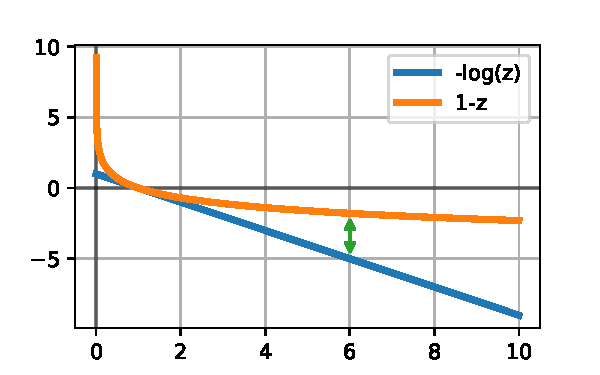
\includegraphics[width=.4\textwidth]{bregmandef.pdf}
	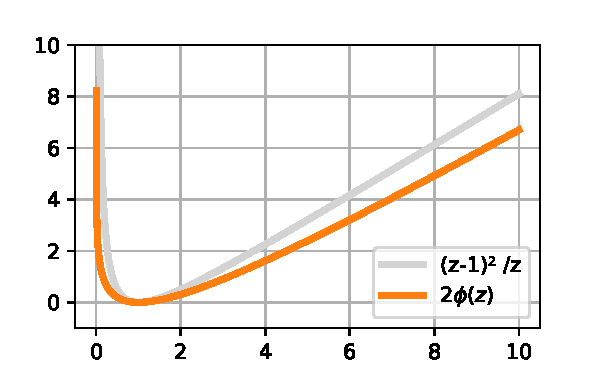
\includegraphics[width=.4\textwidth]{phi.pdf}
	\caption{$\phi(z)$ is the Bregman divergence induced by $-\log(z)$. It is a barrier near $0$. As a result, it is poorly approximated by quadratics.}
	\label{fig:phi}
\end{figure}

\begin{figure}[ht]
	\centering
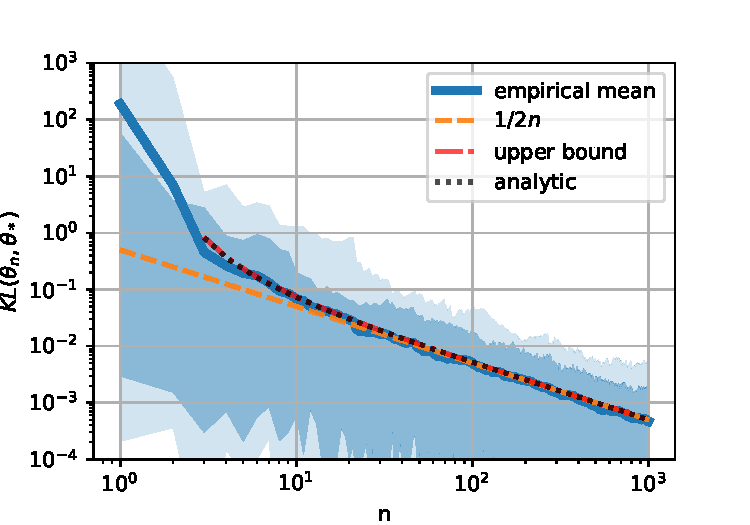
\includegraphics[width=.48\textwidth]{asymptote.pdf}
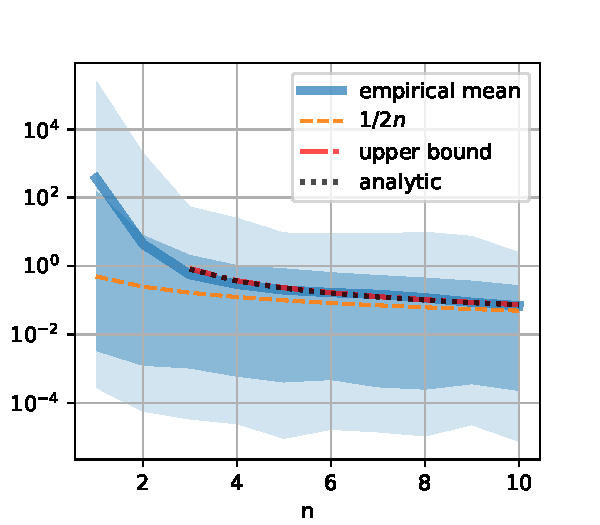
\includegraphics[width=.48\textwidth]{fewsamples.pdf}
	\caption{Suboptimality of a Gaussian variance MLE against number of samples $n$. Bold curve is average over 100 trials,  dark shaded area is 90\% (dark) confidence interval, light shade is min-max interval.  
	\textbf{Left:} as $n$ increases, the suboptimality matches the $1/2N$ asymptote.
	\textbf{Right:} the first few samples significantly deviate from this behavior. In fact, for $n=1$ and $n=2$, the expected value is infinite, but we have a closed form solution and a simple upper-bound for $n>2$.
	}
	\label{fig:curves}
\end{figure}

\bibliographystyle{apalike}
\bibliography{../references.bib}

\end{document}